\documentclass{css}
%\documentclass[noauthor]{css}
%\documentclass[english]{css}

\usepackage[dvips]{graphicx}
\usepackage{latexsym}
\usepackage{color}
\usepackage{moreverb}
\usepackage{cite}

\def\Underline{\setbox0\hbox\bgroup\let\\\endUnderline}
\def\endUnderline{\vphantom{y}\egroup\smash{\underline{\box0}}\\}
%\def\|{\verb|}

\begin{document}

\title{キャッシュを包括するウェブセキュリティモデル}
\etitle{Toward Formal Verification of Web Security with Cache}

\affiliate{osaka-u}{大阪大学\\
Osaka University}
\affiliate{nara}{奈良工業高等専門学校\\
National Institute of Technology, Nara College}

\author{島本 隼人}{Hayato Shimamoto}{osaka-u}
\author{矢内 直人}{Naoto Yanai}{osaka-u}
\author{岡村 真吾}{Shingo Okamura}{nara}
\author{藤原 融}{Toru Fujiwara}{osaka-u}


\begin{abstract}
ウェブの安全性解析として形式手法を用いた手法が提案されている。しかし、この既存研究のモデルには現実のウェブでは欠かせない概念であるキャッシュが含まれていない。実際にBrowser Cache Poinsoning攻撃といったキャッシュを用いたHTTPSに対する攻撃法が存在することから、キャッシュの概念はウェブの安全性解析には不可欠である。本研究では、キャッシュを包括したウェブセキュリティモデルを提案する。提案モデルではキャッシュの概念に加え、その運用を行うHTTPヘッダや中継者の概念も新たに提案する。
\end{abstract}

\begin{jkeyword}
システム,キャッシュ,ウェブセキュリティモデル、セキュリティモデル、形式手法
\end{jkeyword}

\begin{eabstract}
Cache is an important concept in a web system in order to provide them efficiently. Since a browser cache poisoning attack, where an adversary utilizes a web cache, has been proposed recently, analyzing the security under environments with cache is necessary. In this work, we propose a new security model including the cache. We also implement several parts of the model in Alloy.
\end{eabstract}

\begin{ekeyword}
system, cache, web security model, security model, formal method
\end{ekeyword}

\maketitle

\section{はじめに}
\subsection{研究背景}
ウェブ上で個人情報を取り扱う機会の増加にともない,ウェブ通信の解析がより重要となっている.
\color{red}
ウェブの解析はウェブモデルを用いた形式手法により自動化できることから,これらの研究が近年盛んである.
\color{black}
しかし、もしモデルが包括している機能や要件定義が不十分である場合,適切な解析が行えない。
そのため、使用するウェブモデルが適切であることが重要となる。

一般に、安全性要件の解析に使われるモデルはセキュリティモデルと呼ばれる。
セキュリティモデルでは攻撃者の能力,運用する環境などの条件,許容できる被害レベルなどの安全性が定義されており,攻撃者の能力など各パラメータを数値化することで定量的な評価を可能とする.
直観的には満たすべきセキュリティモデルを選択し,実装システムがそのモデルに含まれるかどうかを考察することで,実装モデルの安全性が確認できる.
また,この解析を形式手法ツールを用い自動化することにより,安全性解析にかかる労力を大幅に削減できる.

\color{red}
この形式手法を用いた解析に向けて、Ahkaweらによって提案されたモデル\cite{webmodel}が存在し、このセキュリティ機能を導入した初のモデルである。
\color{black}
\color{red}
(引用つける)
\color{black}
しかしながら本研究ではAhkaweらのモデルにはキャッシュの概念が含まれていないことを指摘する.
現在,キャッシュはその利便性から広く使われている技術であり,ウェブの安全性を考える上で欠かすことができない.
事実,キャッシュを利用した攻撃法も近年の成果において報告されている\cite{bcpattack}.
以上のことから本研究はキャッシュの動作を包括するウェブセキュリティモデルの提案を目的とする。

\subsection{貢献}
\color{red}
本研究で提案するウェブセキュリティモデルはウェブで使用するキャッシュの動作を、格納と再利用、再利用の可能性判定、レスポンスの検証の三点に分けて包括する。
また、ウェブ上でキャッシュを搭載しうる存在としてクライアントとウェブサーバに加えて中継者があり、提案モデルではキャッシュの動作に必要な要素として導入している。
さらに、キャッシュを実際に利用する際に必要となるHTTP ヘッダも新たに導入する。
例えば、キャッシュの動作の指定に必要なCache-Controlヘッダや有効期限の計算に必要となるレスポンスの生成時刻を記述するDateヘッダである。

この提案モデルの一部を形式手法ツールAlloyを用いて実装している。
また、Alloyの機能を用いて、実装を終えた部分についてはHTTPの仕様に従って正常に実装ができているかを確認している。
\color{black}

\subsection{関連研究}
Ahkaweらによる既存モデル\cite{webmodel}は本研究で提案するウェブセキュリティモデルのベースとなっている。
このモデルはBauらによる昨今の形式手法を用いた研究の調査論文\cite{security_modeling_and_analysis}においても取り上げられており、
現在のウェブ環境においてよく使用されるHTTPやDNSといった概念を包括し、現在のウェブの環境に最適なものである。
しかしこのモデルにはキャッシュが包括されていない。
この既存モデルの詳細は\ref{sec:existingmodel}節に記述する。
また、キャッシュを用いた攻撃法としてブラウザキャッシュ汚染攻撃~\cite{bcpattack}が報告されており、提案モデルの能力評価に使用する。
この攻撃法の詳細についても\ref{sec:problem}節に記述する。
加えて、SSL/TLSの安全性についての研究\cite{securing_frame_communication_in_browsers}があり、この研究で想定されている攻撃者の能力を提案モデルが含む脅威モデルとして利用している。

形式手法を用いた研究として、耐タンパー性を持つソフトウェアの動作を行うハードウェアの検証\cite{specifying_and_verifying_hardware_for}があり、形式手法が脆弱性とその対策に有効であることが示されている。
\color{red}
同様に、ウェブにおけるXMLの機能を拡張するWeb Services Enhancements(WSE)やWindowsにおいて通信APIとして使用されるWindows Communication Foundation(WCF)、Extensibe Markup Language(XML)に必要な安全性要求を形式手法を用いて発見した研究\cite{TFFWS27,TFFWS28}がある。
\color{black}
また、OSカーネルの検証\cite{sel4_formal_verification_of_an}が形式手法を用いて行われており、形式手法を安全性証明として利用できることを示している。
さらに、形式手法はAndroidOSの検証\cite{towards_formal_analysis_of_the}にも利用されている。この研究はOSのユーザ権限に着目した安全性検証を目指している。
これらの他に形式手法は様々な対象に応用されており、アルゴリズムやプロトコルの安全性検証に用いられており、暗号アルゴリズムやSSL3.0、鍵交換プロトコル、認証プロトコルに対する検証が存在する\cite{TFFWS17,TFFWS18,TFFWS19,TFFWS20}。
\color{red}
また、本研究では形式手法ツールAlloyを用いており、このAlloyを用いている研究としてアプリケーションのアクセスパターンに着目した安全性の検証を行う研究\cite{finding_security_bugs_in_web}が存在する。
\color{black}

\color{red}
(関連研究追加する)
\color{black}

\section{Ahkaweらのモデルの問題}

\subsection{モデルの概要}
\label{sec:existingmodel}
\color{red}
(余裕があれば関連研究へ)
\color{black}

Ahkaweらによる既存モデル\cite{webmodel}に包括されている概念は大きく三つである。
一つ目はブラウザである。
ブラウザはクライアントとしての基本的な動作とCookieやスクリプトなどの動作が想定されている。
二つ目はウェブサーバである。
ウェブサーバではHTTPレスポンスに対応する動作とDNSに対応する動作の二点に注目している。
また、ネットワークの末端に位置しIPアドレスを保有するしていることが想定されている。
三つ目はネットワークである。
ネットワークには通信プロトコルや、それに必要な要素が包括される。
既存モデルではHTTPやHTTPS、DNSが包括されており、これらの運用に必要となるHTTPヘッダや認証局(CA)なども含まれる。

また、既存モデルでは三種類の脅威モデルが想定されている。
一つ目はweb attackerと呼ばれる攻撃者である。
web attackerは最も基本的な攻撃能力を持つ攻撃者であり、以下の能力を有する。
\begin{itemize}
\item 任意のHTTPリクエストの送信
\item 管理するウェブサーバでの任意のレスポンスの生成
\item 所有するドメインの正当なサーバ証明書の生成
\end{itemize}
二つ目のnetwork attackerはweb attackerの能力に加えて暗号化されていない通信の盗聴と改ざん、自己署名サーバ証明書を用いたなりすましの能力を持つ。
三つ目のgadget attackerはweb attackerの能力に加えてハイパーリンクや画像といった特定の形式のコンテンツを通信内容に挿入できる能力を持つ。

\subsection{モデルの潜在的脆弱性}
\label{sec:problem}
Ahkaweらによる既存モデル\cite{webmodel}では、キャッシュの概念が包括されていない。
キャッシュはウェブサーバからクライアントへ送信されたレスポンスを保存する領域を持ち、そのレスポンスの再利用によって通信時間を短縮でき通信の効率化をおこなえる。
このような利点からキャッシュは現在広く使用されている。

一方で、キャッシュを利用した攻撃法としてブラウザキャッシュ汚染攻撃(BCP攻撃)~\cite{bcpattack}を紹介する。
BCP攻撃は中間者攻撃の一つであり、ウェブサーバから送信されるレスポンスを中間者攻撃によって改ざんし、ブラウザに搭載されているキャッシュに保存させる。
これにより、改ざんレスポンスがキャッシュからリロードされるため、ブラウザに悪影響を与えることが可能になる。
たとえば、レスポンス内に悪質なサイトのリンクを追加することでブラウザを誘導したり、スクリプトを記述することによりブラウザに任意の動作を強制することができる。
この攻撃法の特徴はキャッシュによるレスポンスの再利用機能を利用することにより、一度の中間者攻撃で長期に渡る悪影響が可能になる点である。
また、この攻撃法はHTTPSに対する攻撃も可能である。
この場合には、攻撃者は中間者攻撃を行う際に自己署名証明書を使用して正当な接続先になりすます必要がある。
このなりすましに使用する自己署名証明書の安全性をブラウザでは確認できないため、ブラウザではユーザに対して認証警告が表示する。
この認証警告をユーザが無視することがHTTPSに対するBCP攻撃の条件である。

このBCP攻撃のようにキャッシュを利用した攻撃法が存在すること、また、加えてキャッシュは一般に使用されているものであることから、ウェブの安全性解析を行う上でキャッシュは必要不可欠な概念である。
したがって、キャッシュを導入したモデルを提案する必要がある。

\subsection{キャッシュを包括するセキュリティモデルにむけて}
キャッシュを導入したモデルの提案に伴って、合わせて必要となる概念がある。
まず、中継者と呼ばれる概念である。
HTTPにおいて、キャッシュはクライアントとウェブサーバの他に中継者に搭載される。
ここで中継者はネットワークの末端のクライアントとウェブサーバの経路上に存在するものであり、具体的にはプロキシやゲートウェイを指す。
プロキシは通信経路を最適化することで通信効率を向上させ、また、クライアントの匿名性を保持するために使用される。
ゲートウェイは内部のネットワークとウェブ(外部ネットワーク)を接続するサーバであり、ゲートウェイで翻訳を行うことにより異なるプロトコルの通信を可能にする。
これらもキャッシュと同じくウェブで広く使用されている要素であるとともに、またキャッシュを使用する概念であることから、キャッシュを導入したモデルを提案する際にはこの中継者の概念も追加する必要がある。
モデルにはこれらに加えて、キャッシュおよび中継者の動作に使用されるヘッダが新たに必要となる。
レスポンスをキャッシュに保存する際に適応するオプションやキャッシュ内での有効期限はレスポンス内のヘッダで指定する。
このヘッダはキャッシュの運用にのみ使用されるヘッダであり、提案モデルには導入しておく必要がある。
同様に、中継者の動作に必要なヘッダについても追加する必要がある。

\section{提案モデルの設計}
\label{sec:proposed}
本研究で提案するウェブセキュリティモデルの特徴はキャッシュ、ヘッダ、中継者の大きく三つに分けて考えることができる。

\subsection{キャッシュのモデル定義}
\label{cache}
提案モデルではキャッシュの基本的な運用に対する動作を包括する。ここで包括する動作は以下の三つに分類できる。

\subsubsection{レスポンスの格納と再利用}
\label{sec:store_reuse}
キャッシュは以下の条件すべてを満たしている場合にレスポンスを保存することができる。
\begin{itemize}
\item キャッシュを禁止するオプションが含まれていない
\item 有効期限を計算可能、もしくは、キャッシュを許可する記述がある
\end{itemize}

また、リクエストが要求しているURIをもつレスポンスを保持しているキャッシュは、以下のいずれかに該当する場合にそのレスポンスを再利用してリクエストに返送することができる。

\begin{itemize}
\item レスポンスが有効期限内
\item 有効期限を過ぎているレスポンスの再利用が許可されている
\item レスポンスが検証済み
\end{itemize}

\subsubsection{キャッシュの検証}
キャッシュにおける検証とは、キャッシュ内のレスポンスに含まれているコンテンツがオリジンサーバ内の最新のコンテンツと一致するかを確認する動作である。
検証が必要になった場合、キャッシュはオリジンサーバに対して``条件付きリクエスト''を送信する。
条件付きリクエストとはヘッダで指定した条件を満たしている場合に完全なレスポンスを返すリクエストである。
この条件にはコンテンツの最終更新時間、もしくは、レスポンス内のEtagヘッダから得られる固有値を使用する。
最終更新時刻を用いる場合にはIf-Modified-Sinceヘッダを、固有値を使用する場合にはIf-None-Matchヘッダを使用した条件付きリクエストを生成する。
通信において問題が発生しなかった場合、このリクエストに対するレスポンスの状態コードは200(OK)もしくは304(Not Modified)が想定される。
200(OK)の場合、キャッシュはキャッシュ内のレスポンスを破棄し、新たに取得したレスポンスを使用する。
このとき格納可能条件を満たしていれば、新しいレスポンスをキャッシュしてもよい。
304(Not Modified)であった場合、キャッシュ内のレスポンスのヘッダを今取得したレスポンスのヘッダに置き換えて再利用する。
このヘッダの置換によりレスポンスの有効期限を延長する。
このヘッダの置換時にWaringヘッダが存在する場合、1xxおよび2xxの値は除去する。
また、同じURIに対するレスポンスが同じキャッシュに複数存在する場合、検証結果として送信されるレスポンスに記述されている検証子に該当するレスポンスのヘッダを置換して再利用する。
複数のレスポンスに該当する場合には、そのレスポンスのうち最新のレスポンスを採用する。

\subsubsection{キャッシュの有効期限}
\label{sec:expiration}
最後は、レスポンスの有効期間の判定である。
この判定にはレスポンスの有効期限と生成されてからの経過時間が必要となる。
まず、キャッシュは以下の値を有効期間として採用する。
複数個存在する場合にはより上位に書かれている値を採用する。
\begin{enumerate}
\item キャッシュが共有キャッシュでありs-maxageが存在する場合、s-maxageの値
\item max-ageが存在する場合、max-ageの値
\item Expiresヘッダが存在する場合、(Expiresの値 - Dateヘッダの値)で求められる値
\end{enumerate}
もし、同項目に複数個の値が示されている場合、例えば、max-ageに異なる値が2つ以上記述されている場合には、そのレスポンスは常に有効期限切れとして扱う。
また、上記のどの値も得られなかった場合、キャッシュは任意の期限を設定する。
この期限の設定ではLast-Modifiedヘッダの値を用いて計算することが多い。

次に、キャッシュが経過時間を計算するには以下の値が必要となる。
\begin{eqnarray*}
age & = & \mbox{Ageヘッダの値}\\
date & = & \mbox{Dateヘッダ値}\\
current & = & \mbox{現在時刻}\\
reqtime & = & \mbox{リクエストの受信時刻}\\
restime & = & \mbox{格納レスポンスの受信時刻}
\end{eqnarray*}
これらの値を用いて、経過時間$T_{age}$は以下の手順で計算される。
\begin{eqnarray*}
T_{apparent} & = & max(0,\;restime - date)\\
T_{corrected} & = & age + (restime - reqtime)\\
T_{initial} & = & max(T_{apparent},\;T_{corrected})\\
T_{visit} & = & current - restime\\
T_{age} & = & T_{initial} + T_{visit}
\end{eqnarray*}

\subsection{ヘッダのモデル定義}
提案モデルでは、キャッシュおよび中継者の動作に必要となるヘッダを新たに包括する。
表\ref{tb:model_header}にその一覧を示す。

\begin{table}[htb]
\centering
\caption{提案モデルで追加するHTTPヘッダ}
\label{tb:model_header}
\begin{tabular}{c|c}
\hline
HTTPヘッダフィールド & HTTPヘッダ \\ \hline \hline
HTTPRequestHeader & IfModifiedSinceHeader \\
 & IfNoneMatchHeader \\
 & PragmaHeader \\ \hline
HTTPResponseHeader & AgeHeader \\
 & EtagHeader \\
 & LastModifiedHeader \\ \hline
HTTPGeneralHeader & CacheControlHeader \\
 & ConnectionHeader \\
 & DateHeader \\
 & WarningHeader \\ \hline
HTTPEntityHeader & ExpiresHeader \\ \hline
\end{tabular}
\end{table}

ヘッダフィールドはヘッダを用途と役割によって分類する。
Ahkaweらによる既存モデル\cite{webmodel}では、HTTPRequestHeaderとHTTPResponseHeaderが含まれており、これらに加えて提案モデルではHTTPGeneralHeaderとHTTPEntityヘッダを追加している。
この四種類の分類はHTTPの仕様においても用いられている。
HTTPRequestHeaderとHTTPResponseHeaderはそれぞれ、リクエストもしくはレスポンスでのみ使用可能なヘッダが属する。
これに対して、HTTPGeneralHeaderとHTTPEntityHeaderはリクエストとレスポンスのどちらにも使用可能なヘッダが属しており、この二つの違いは属するヘッダの役割である。
HTTPGeneralHeaderに含まれるヘッダはリクエストやレスポンスそのものの情報を表す。
例えば、レスポンスのサーバにおける生成日時を記録するために用いられる。
一方で、HTTPEntityHeaderに属するヘッダはリクエストやレスポンスに含まれているコンテンツの情報を表す。
例えば、レスポンスで送信されているファイルの最終更新日時をクライアントに伝達するといった役割を担う。

また、表\ref{tb:model_header}に含まれているヘッダのうち、特に重要な役割をもつ一部のヘッダを説明する。
一つ目としてCache-Controlヘッダが考えられる。
このヘッダは様々なオプションの記述によって、キャッシュの動作を指定することができる点で、キャッシュの動作に強く影響を与えるヘッダであるという点で重要である。
使用するオプションの一例としてmax-ageがあり、非負整数を記述することでレスポンスがキャッシュに格納された際の有効期限を指定することができる。
また、キャッシュへの保存を許可しないno-store、検証を行わないレスポンスの再利用を許可しないno-cacheといったキャッシュの動作に制限を与えるオプションも存在する。

次に、キャッシュ内のレスポンスが再利用可能か判定するために必要なヘッダについて考える。
再利用可能判定では、レスポンスの有効期限と生成からの経過時間が必要となり、経過時間の計算は\ref{cache}節において前述した計算式を用いる。
したがって、この計算で用いるDateヘッダ、Ageヘッダはレスポンスの再利用可能判定に必須であり重要なヘッダである。
Dateヘッダはレスポンスのオリジンサーバにおける生成時刻、Ageヘッダはレスポンスの生成からの経過時間を表す。

最後にキャッシュの検証機能に必要なヘッダを考える。
検証の動作はコンテンツの最終更新時間を用いる手法と、固有値を用いる手法の二種類が存在する。
最終更新時間を用いる検証には、最終更新時間を記述するLastModifiedヘッダと、記述されている時刻以降の更新が行われている場合にコンテンツの再送信を求めるIf-Modified-Sinceヘッダが必須である。
また、固有値を用いる検証には、固有値を伝達するEtagヘッダと、記述されている固有値と最新のコンテンツの固有値が異なる場合に再送信を求めるIf-None-Matchヘッダが必要である。

提案モデル内には、役割が重複しているヘッダも存在している。
例えば、Expiresヘッダはレスポンスの有効期限を、Pragmaヘッダはno-cacheのオプションを表すことができるが、これらはCache-Controlヘッダを使用することでも表現可能である。
これは、Cache-ControlヘッダがHTTP/1.1で新しく追加されたものであるからであり、HTTP/1.1においてはExpiresヘッダ、および、Pragmaヘッダの使用は推奨されていない。
この二つのヘッダは、HTTP/1.1が動作していない環境のみの使用が想定されてい
しかし、既存モデルはHTTP/1.0とHTTP/1.1の両方を含む環境を想定しているため、提案モデルにおいてもこの想定環境を引き継ぐことを目的としてこの二つのヘッダを包括している。

\subsection{ウェブ要素のモデル定義}
提案モデルでは、包括しているウェブの構成要素を図\ref{fig:model_header}のように構成している。
図\ref{fig:model_header}において、濃く表示している要素は提案モデルで新たに追加した概念であり、矢印はクラスの継承構造を表す。

図\ref{fig:model_header}の一番上に存在するNetworkEndpointはネットワークの末端に存在する要素の概念を表し、HTTPConfirmistはHTTPの仕様に従う動作をする概念を表す。
既存モデルでは、クライアントとウェブサーバがこの概念に含まれており、この二つと並列に中継者の概念(HTTPIntermediate)を追加している。
さらに中継者はプロキシ(HTTPProxy)とゲートウェイ(HTTPGateway)の概念を内包している。

HTTP/1.1においてプロキシは通過するコンテンツへの編集と通信経路の設定の二つの機能を持つが、これらの機能はキャッシュの機能に大きな影響は与えない。
提案モデルはキャッシュの動作に注目した安全性検証を目的としているため、プロキシを通信経路上に存在するキャッシュを搭載する要素とみなす。

ゲートウェイは外部ネットワークからHTTPを用いてアクセスされる場合、ウェブサーバとして認識され同様の動作を行う。
このことから、提案モデルではゲートウェイの内部ネットワークにおける動作は考慮せず、ウェブサーバとみなして設計する。

\begin{figure}[htb]
\centering
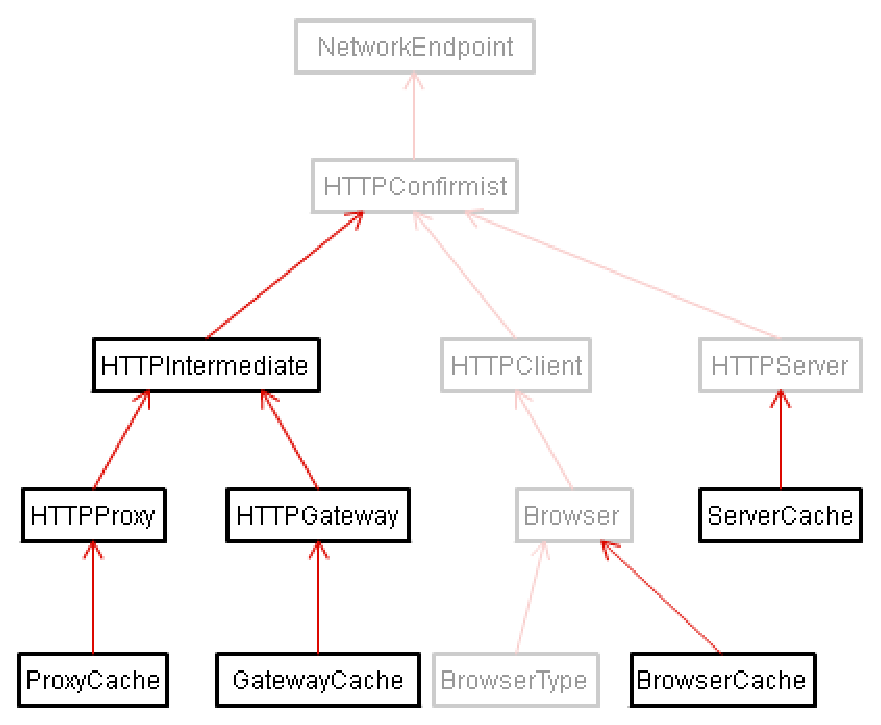
\includegraphics[width=0.8\hsize]{model_archi.eps}
\caption{提案モデルに含まれるウェブアーキテクチャ}
\label{fig:model_header}
\end{figure}

\section{モデル実装}
提案モデルの実装は形式手法ツールであるAlloyを用いて進めている。
\color{red}
Alloyはモデルを与えて実行することで、そのモデルがとり得る状態をすべて出力する。
この出力された状態が安全であるかを確認することで、システムの安全性を証明することができると同時に、潜在的な危険性の発見が可能である。
また、出力する状態を限定する条件を設定することができ、システムがとってはならない動作を条件として設定することで、その状態に至る原因の発見にも役立つ。
\color{black}
Ahkaweらによる既存モデル\cite{webmodel}はこのAlloyを用いて実装が行われており、提案モデルはこれを拡張して実装を進める。

\color{red}
実装を行う項目と実装を終えている項目を表\ref{tb:model_implement}に示す。
また、モデルにおける実装済みの項目の構造は図\ref{fig:model_alloy}のように表される。
図\ref{fig:model_alloy}内の黒の矢印は継承関係を表し、その他の色は集合ごとの関係性を表す。
例えば、Generalヘッダフィールドに属しているCache-Controlヘッダは、モデル内ではHTTPGeneralHeaderをCacheControlHeader継承している関係性で表現されている。
また、Cache-Controlヘッダとそのオプションを表すCacheOptionはoptionsと関連付けられている。

\begin{table}[htb]
\centering
\caption{実装項目}
\label{tb:model_implement}
\begin{tabular}{l|c}
実装項目 & 実装済み \\ \hline
レスポンスの格納 & ○ \\
レスポンスの再利用 & ○ \\
レスポンスの検証機能 & - \\
中継者 & - \\
ヘッダ & △(一部) \\
\end{tabular}
\end{table}

\begin{figure}[htb]
\centering
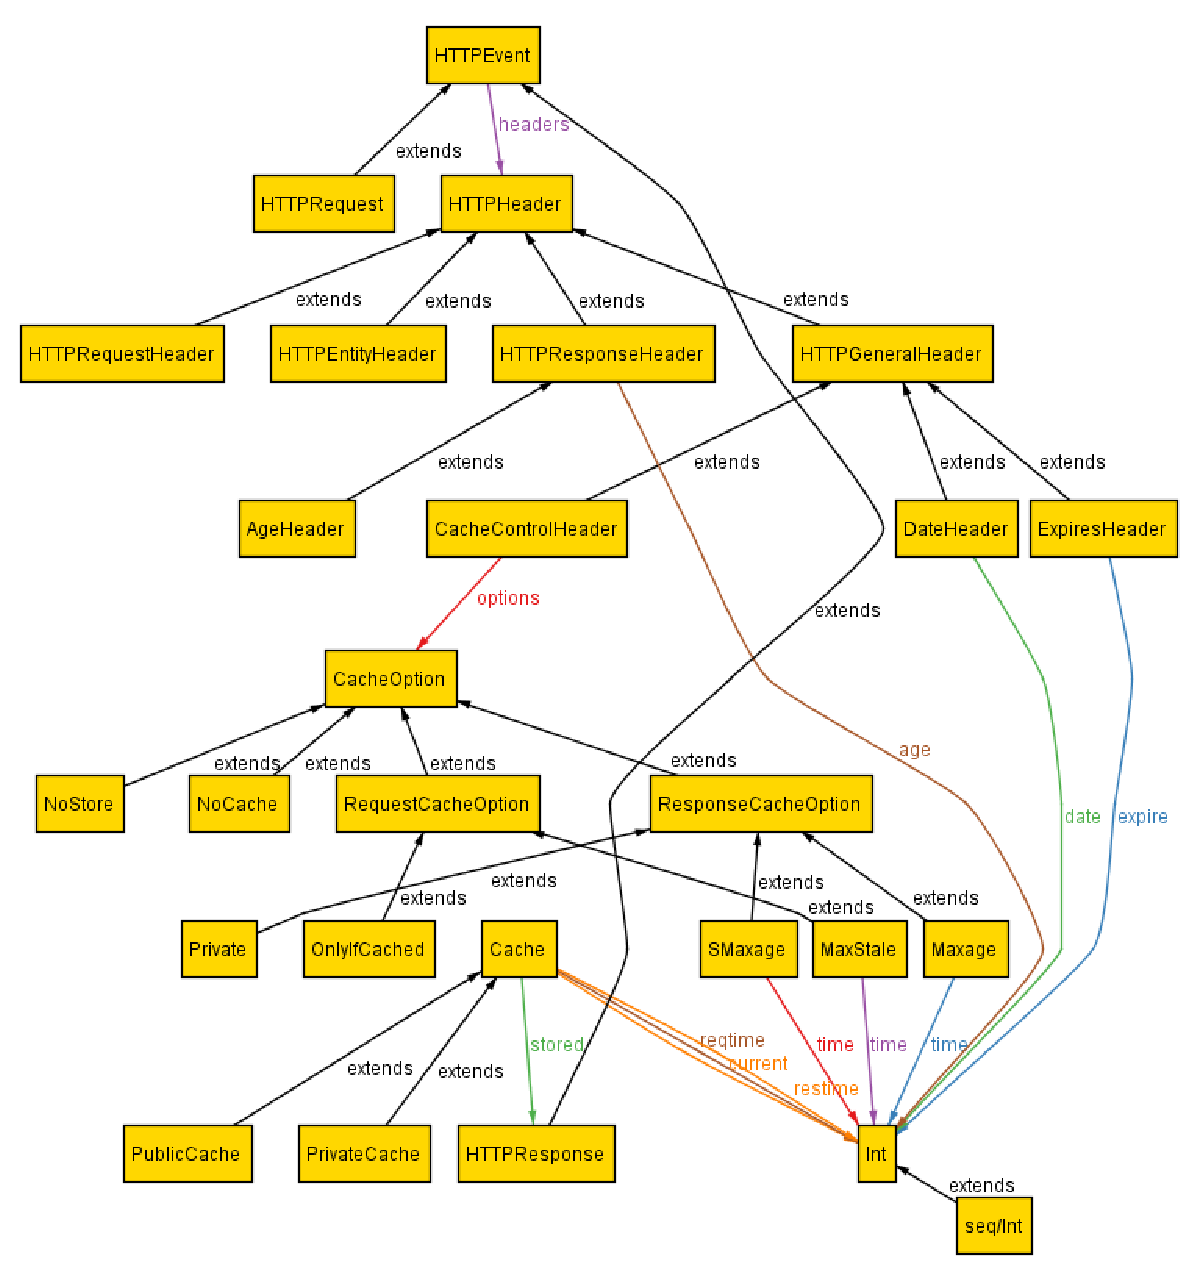
\includegraphics[width=1.0\hsize]{model_alloy.eps}
\caption{実装中の提案モデル}
\label{fig:model_alloy}
\end{figure}

提案モデル内で整数値はIntクラスを関連付けることで表現できる。
例えば、CacheControlヘッダのmax-ageのようないくつかのオプションには整数値を用いるものが存在し、このようなオプションにIntクラスが関連付けられていることが図\ref{fig:model_alloy}に示している。
同様に、日時を表す値を必要とするDateヘッダにもIntを関連付けている。
本来、日時を表す値と整数値は異なるものであるが、HTTPにおいて日時を表す値を用いる際には対応する整数値に変換して扱うため、Intクラスを関連付けることはHTTPの仕様に反してはいない。

これらの整数値を持つクラスはレスポンスの有効期限の条件の記述に利用している。\\\hrulefill
\begin{small}
\begin{verbatimtab}[3]
1:	let A = HTTPResponse.headers.age, 
	D = HTTPResponse.headers.date |
2:		let apparent=(restime.minus[D]>0 implies
		restime.minus[D] else 0), corrected = 
		A.plus[restime.minus[reqtime]] | 
3:			let initial=(apparent>corrected 
			implies apparent else corrected) | 
4:				Maxage.time.minus[initial.plus
				[current.minus[restime]]]>0
\end{verbatimtab}
\end{small}
\hrulefill\\
このコードは、PrivateCacheにおけるmax-ageの値を有効期限に採用する際に満たしているべき条件、つまり、
\ref{sec:expiration}節における計算を行いその値がmax-ageの値よりも小さいことを示している。

また、表\ref{tb:model_implement}の未実装の項目は、現在実装を進めており今後の課題である。
\color{black}

\section{実装モデルの正当性}
提案モデルのヘッダ定義が正当であることを確認する。
前述した通り実装モデルを与えてAlloyを動作させると、そのモデルを満たす状態が出力される。
本章では、出力された状態がHTTPの仕様を満たしていることを確認することで、正当性を考察する。

\subsection{レスポンスの格納と再利用}
図\ref{fig:case1}が表す状態aでは、あるHTTPリクエストに対して個別キャッシュに格納されているレスポンスを再利用し応答することが可能であることが示されている。

\begin{figure}[htb]
\centering
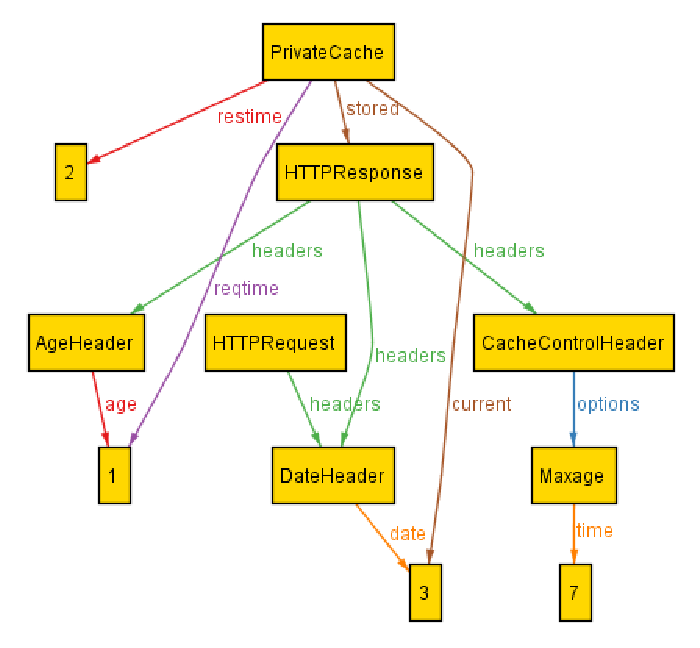
\includegraphics[width=1.0\hsize]{case1.eps}
\caption{状態a}
\label{fig:case1}
\end{figure}

図\ref{fig:case1}より、このHTTPリクエストのヘッダは以下のように想定されている。
\begin{verbatimtab}[4]
	Date: 3
\end{verbatimtab}
同様に、HTTPレスポンスは以下のヘッダが想定されている。
\begin{verbatimtab}[4]
	Date: 3
	Age: 1
	Cache-Control: max-age=7
\end{verbatimtab}
ここで、このレスポンスのキャッシュへの格納、およびこの状況における再利用が正当であるかを考察する。
まず、このレスポンスにはキャッシュを禁止する記述はなく、かつ、有効期限を明記するCache-Controlヘッダのmax-ageオプションが指定されているため、\ref{sec:store_reuse}節のキャッシュへの格納条件を満たしている。
次に、\ref{sec:expiration}節のキャッシュの再利用条件について考察する。
レスポンスのヘッダに有効期限を過ぎているレスポンスの再利用を許可する記述はなく、キャッシュの検証も行っていないため、レスポンスが有効期限内である必要があり図\ref{fig:case1}の情報から判定を行う。
有効期限はmax-ageの値が採用され7となり、レスポンスの経過時間$T_{age}$を\ref{sec:expiration}節の計算式を用いて求める。
\begin{eqnarray*}
&&age\;=\;1,\; date\;=\;3,\; current\;=\;3\\
&&reqtime\;=\;1,\; restime\;=\;2\\
&&T_{apparent}\;=\;max(0,\;restime - date)\;=\;0\\
&&T_{corrected}\;=\;age + (restime - reqtime)\;=\;2\\
&&T_{initial}\;=\;max(T_{apparent},\;T_{corrected})\;=\;2\\
&&T_{visit}\;=\;current - restime\;=\;1\\
&&T_{age}\;=\;T_{initial} + T_{visit}\;=\;3
\end{eqnarray*}
以上より経過時間は有効期限内となり、レスポンスは再利用可能条件を満たしている。
したがって、状態aはHTTPの仕様を満たしている。

\color{red}
\subsection{Privateオプション}
以下のコマンドにより、Privateオプションが記述されている際に共有キャッシュにレスポンスが格納されていないかを確認できる。
実行の結果、共有キャッシュにレスポンスが格納されている反例が存在しなかったため、Privateオプションは正常に動作している。\\\hrulefill
\begin{small}
\begin{verbatimtab}[2]
assert checkPrivate{
	#Private>0 implies #PublicCache.stored=0
}
check checkPrivate for 10
\end{verbatimtab}
\end{small}
\hrulefill

\subsection{No-storeオプション}
以下のコマンドにより、No-storeオプションが記述されている際にキャッシュにレスポンスが格納されていないかを確認できる。
実行の結果、キャッシュにレスポンスが格納されている反例が存在しなかったため、No-storeオプションは正常に動作している。\\
\hrulefill
\begin{small}
\begin{verbatimtab}[2]
assert checkNoStore{
	#NoStore>0 implies #Cache.stored=0
}
check checkNoStore for 10
\end{verbatimtab}
\end{small}
\hrulefill

\color{black}

\section{結論}
本研究では,Ahkaweらの既存のウェブセキュリティモデル\cite{webmodel}に不足点があることを受けて、新たにキャッシュを含むセキュリティモデルを提案した。
主にキャッシュの動作,キャッシュを搭載するウェブの構成要素,キャッシュの動作に使用するヘッダについてHTTP/1.1及びHTTP/1.0の仕様に従ってモデルを作成した.
また,提案モデルの実装を行っており、実装を終えている機能についての正当性の確認を行った.
その結果、レスポンスの格納や再利用、その条件判定について正常に動作していることを確認した。

本研究の今後の課題は、実装を終えていない要素の実装である。
また、この提案モデルの実装後は、現在研究が進められているプロトコルであるHTTP Strict Transport Security (HSTS)\cite{rfc6797}およびPublic Key Pinning for HTTP (HPKP)\cite{rfc7469}を包括したモデルの提案を考えている。
これら二つのプロトコルは暗号通信のプロトコルとして現在広く使用されているHTTPSに含まれる脆弱性を補ったものであり、動作の実装にキャッシュを使用しているため提案モデルとの関連性は高い。
HSTSとHPKPの運用には専用のヘッダを必要とし、モデルではそれらを包括できていない。
しかし、この部分の拡張によってこの二つのプロトコルを包括できる可能性が高いと考えている。

\begin{acknowledgment}
本研究の一部は,JSPS科研費16K16065の助成を受けている.
\end{acknowledgment}

\bibliographystyle{ipsjunsrt}
\bibliography{list}

\end{document}
